\documentclass[journal, spanish]{IEEEtran}

% Paquetes necesarios
\usepackage[T1]{fontenc}
\usepackage[utf8]{inputenc}
\usepackage{babel}
\usepackage{cite}
\usepackage{graphicx}
\usepackage{float}

\title{ Big-O notation}
\author{Juan Esteban Pinzon Preciado \thanks{} \\
\textit{Fundación Universitaria Konrad Lorenz} \\
}

\begin{document}

\maketitle

\section{Introducción}

A fin de comprender el rendimiento y la eficiencia de un conjunto de algoritmos, es crucial llevar a cabo un análisis detallado de su complejidad temporal. Este análisis se realiza comúnmente utilizando la notación Big-O, que nos proporciona una visión general de cómo aumenta el tiempo de ejecución de un algoritmo a medida que crece el tamaño de entrada.

\section{Ejercicio de análisis de complejidad de algoritmos}
En esta sección se describirá la metodología utilizada.

\subsection{Código número uno}
 La inicialización int i = 0;es una operación de tiempo constante, O(1). La condición i < n` se evalúa n veces y la operación i++ se ejecuta n veces. Por lo tanto, la complejidad de este bucle for es O(n).

 Complejidad de O(n)

\begin{figure}[H]
  \centering
  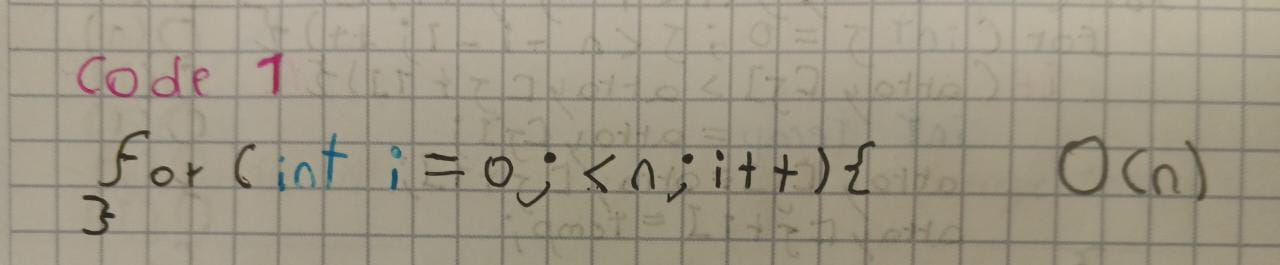
\includegraphics[width=0.5\textwidth]{WhatsApp Image 2023-09-11 at 7.54.49 PM.jpeg}
  \caption{Ejemplo código 1}
  
  \label{fig:imagen1}
\end{figure}


\subsection{Código número dos}
Para el bucle externo \texttt{for}, la complejidad es $O(n)$ debido a que la inicialización y la operación de incremento son de tiempo constante.

Para el bucle interno, la complejidad es $O(m)$ debido a que la inicialización y la operación de incremento también son de tiempo constante. En el contexto del bucle externo, esto resulta en una complejidad total de $O(n) + O(m)$.

Completitud de $O(n)$:
\begin{figure}[H]
  \centering
  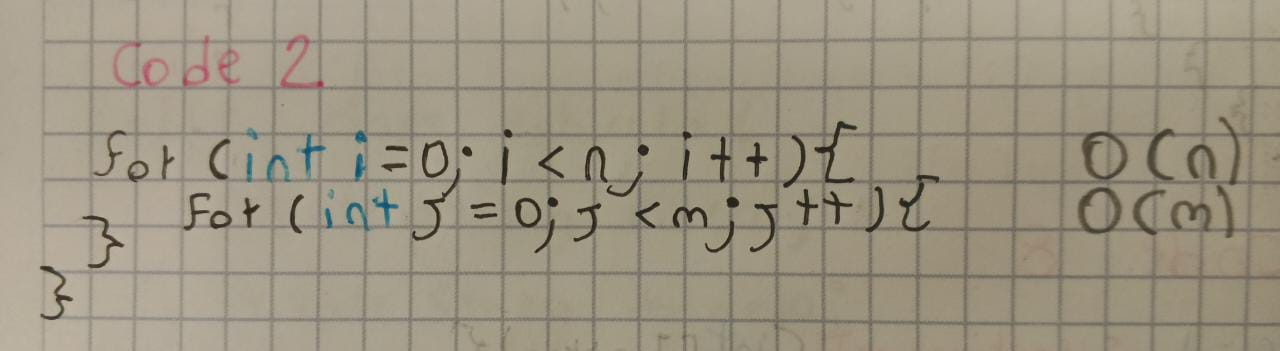
\includegraphics[width=0.5\textwidth]{WhatsApp Image 2023-09-11 at 7.55.14 PM.jpeg}
  \caption{Ejemplo código 2}
  \label{fig:imagen2}
\end{figure}

\subsection{Código número tres}
La línea representa un bucle que se ejecuta "n" veces, por lo que su complejidad es $O(n)$.
El bucle interno se ejecuta en un patrón triangular, realizando aproximadamente $n^2$ iteraciones en total.
Por lo tanto, la complejidad del bucle interno es $O(n^2)$.esto resulta en una complejidad total de $O(n) + O(n^2)$.

Complejidad de $O(n^2)$:
\begin{figure}[H]
  \centering
  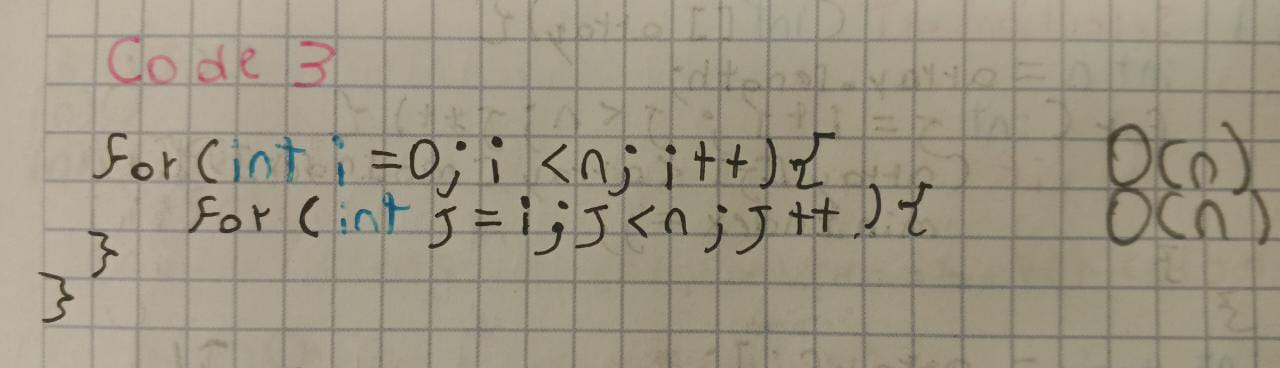
\includegraphics[width=0.5\textwidth]{WhatsApp Image 2023-09-11 at 7.57.25 PM.jpeg}
  \caption{Ejemplo código 3}
  \label{fig:imagen3}
\end{figure}


\subsection{Código número cuatro}

1. La línea `int index = -1;` es una asignación de tiempo constante: O(1).

2. El bucle `for (int i = 0; i < n; i++)` itera sobre un arreglo `array` de longitud `n`, lo que da como resultado una complejidad en el peor caso de O(n).

3. Dentro del bucle, la comparación `if (array[i] == target)` es una operación de tiempo constante y, en el peor caso, se realiza hasta `n` veces: O(n).

4. La asignación `index = i;` es una operación de tiempo constante y se ejecuta una vez en el peor caso: O(1).

5. El `break;` se ejecutará una vez cuando se encuentre el elemento buscado, lo que también es una operación de tiempo constante en el peor caso: O(1).\\

Complejidad de O(n)

\begin{figure}[H]
  \centering
  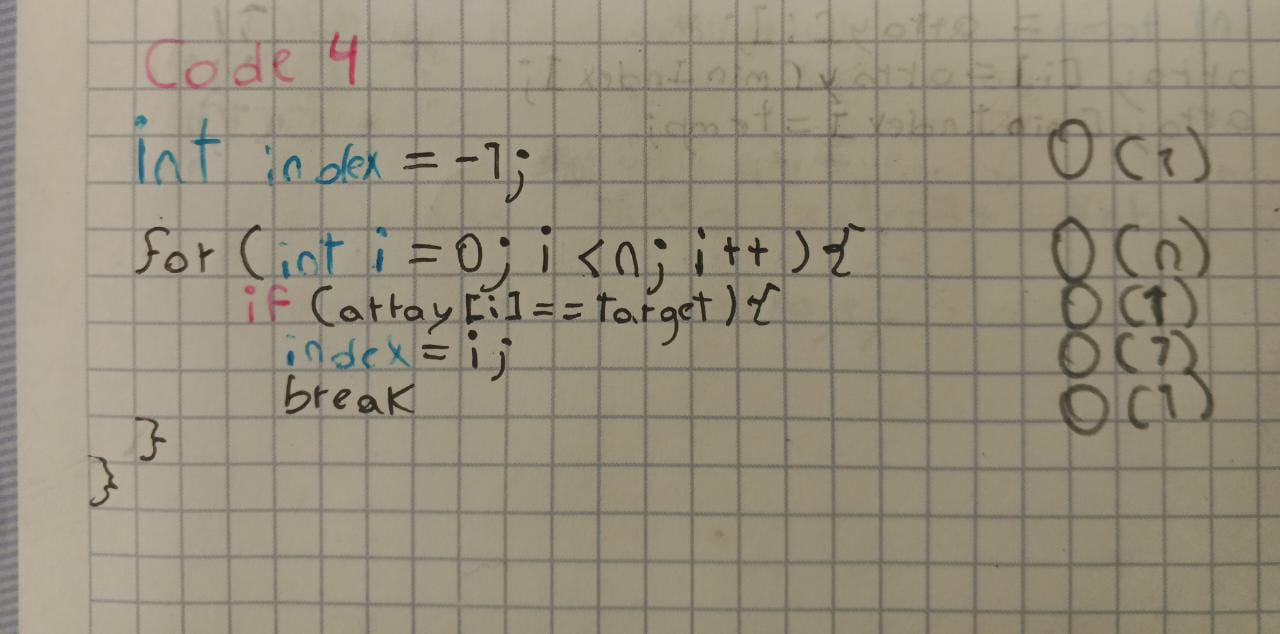
\includegraphics[width=0.5\textwidth]{WhatsApp Image 2023-09-11 at 7.59.47 PM.jpeg}
  
  \caption{Ejemplo código 4}
  \label{fig:imagen1}
\end{figure}\\
  

\subsection{Código número cinco}
1. La línea es una serie de asignaciones de tiempo constante: O(1).

2. El bucle `while (left <= right)` implementa la búsqueda binaria. La búsqueda binaria tiene una complejidad de tiempo de O(log n) .

3. La línea  calcula el índice medio del rango actual. Esta operación es de tiempo constante: O(1).

4. La comparación es una operación de tiempo constante y se ejecuta en el peor caso una vez: O(1).

5. Las asignaciones son operaciones de tiempo constante que también se ejecutan en el peor caso una vez: O(1).

6. El `break;` se ejecutará una vez cuando se encuentre el elemento buscado : O(1).\\

Complejidad de O(log n) 



\begin{figure}[H]
  \centering
  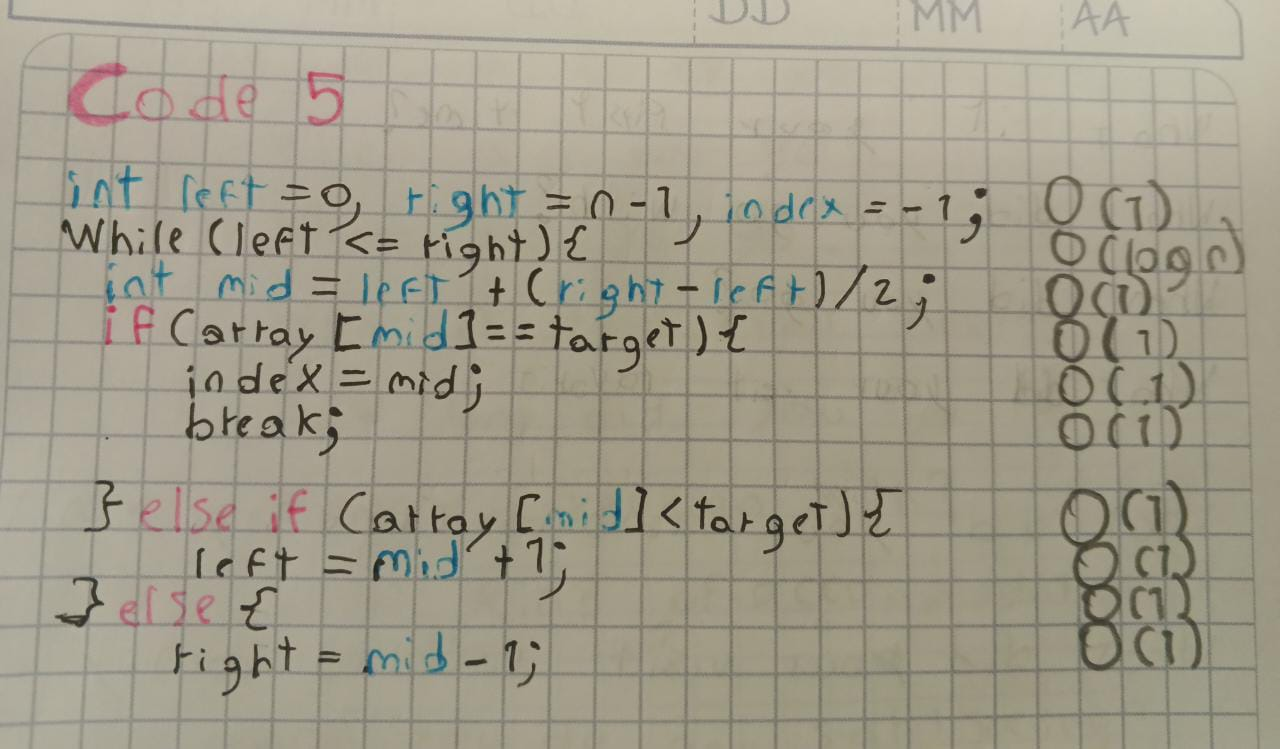
\includegraphics[width=0.4\textwidth]{WhatsApp Image 2023-09-11 at 8.00.07 PM.jpeg}
  \caption{Ejemplo código 5}
  \label{fig:imagen1}
\end{figure}

\subsection{Código número seis}
1. La línea es una serie de asignaciones de tiempo constante: O(1).

2. El bucle `while se ejecutará hasta que `row` sea mayor o igual al número de filas de la matriz `matrix` y `col` sea mayor o igual a cero. En el peor caso, este bucle se ejecutará un máximo de `m + n` veces, donde `m` es el número de filas y `n` es el número de columnas de la matriz. O(n)

3. La comparación if es una operación de tiempo constante y se ejecuta en el peor caso una vez: O(1).

4. Las asignaciones  son operaciones de tiempo constante que también se ejecutan una vez: O(1).

5. Las asignaciones son operaciones de tiempo constante que se ejecutan en el peor caso una vez: O(1).

6. El `break;` se ejecutará una vez cuando se encuentre el elemento buscado: O(1)\\

Complejidad de O(n)

\begin{figure}[H]
  \centering
  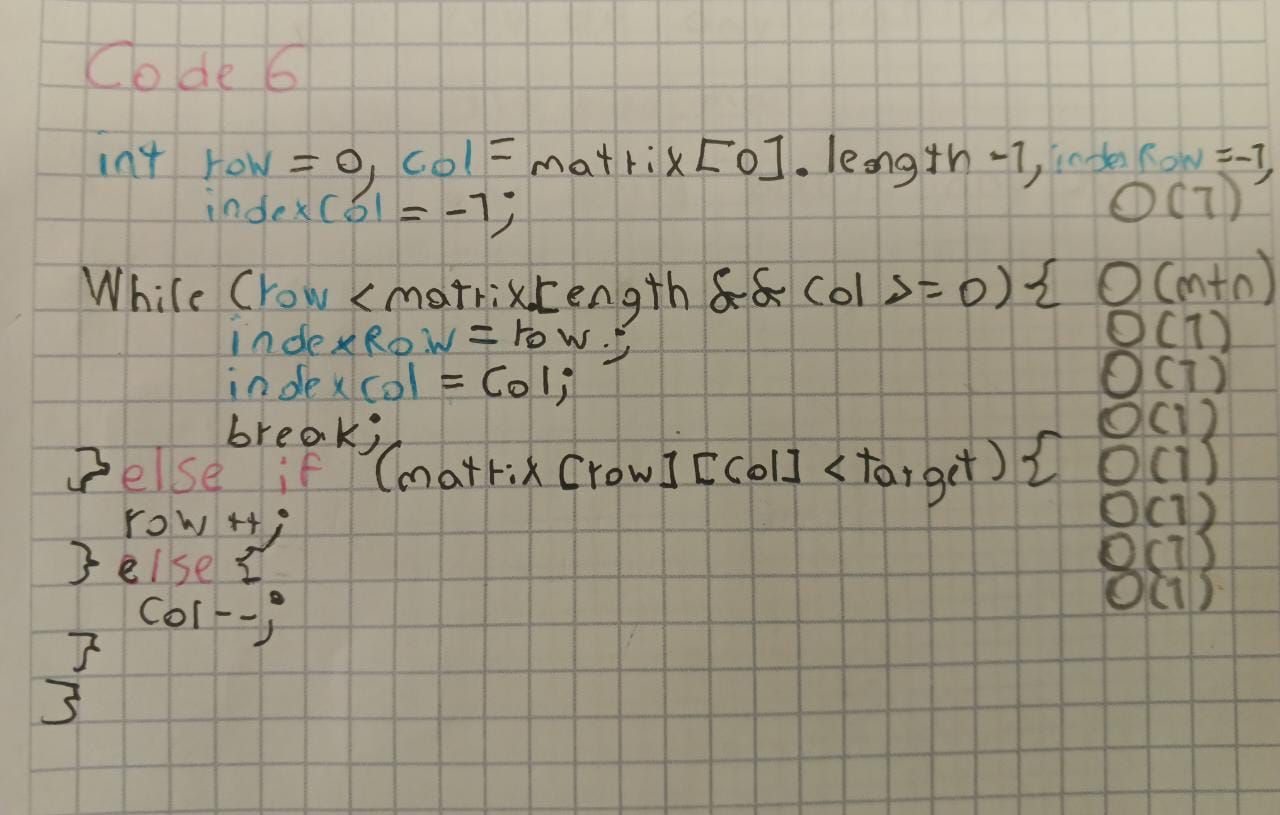
\includegraphics[width=0.4\textwidth]{WhatsApp Image 2023-09-11 at 8.00.24 PM.jpeg}
  \caption{Ejemplo código 6}
  \label{fig:imagen1}
\end{figure}


\subsection{Código número siete}
Aquí se explicará el proceso A.

\begin{figure}[H]
  \centering
  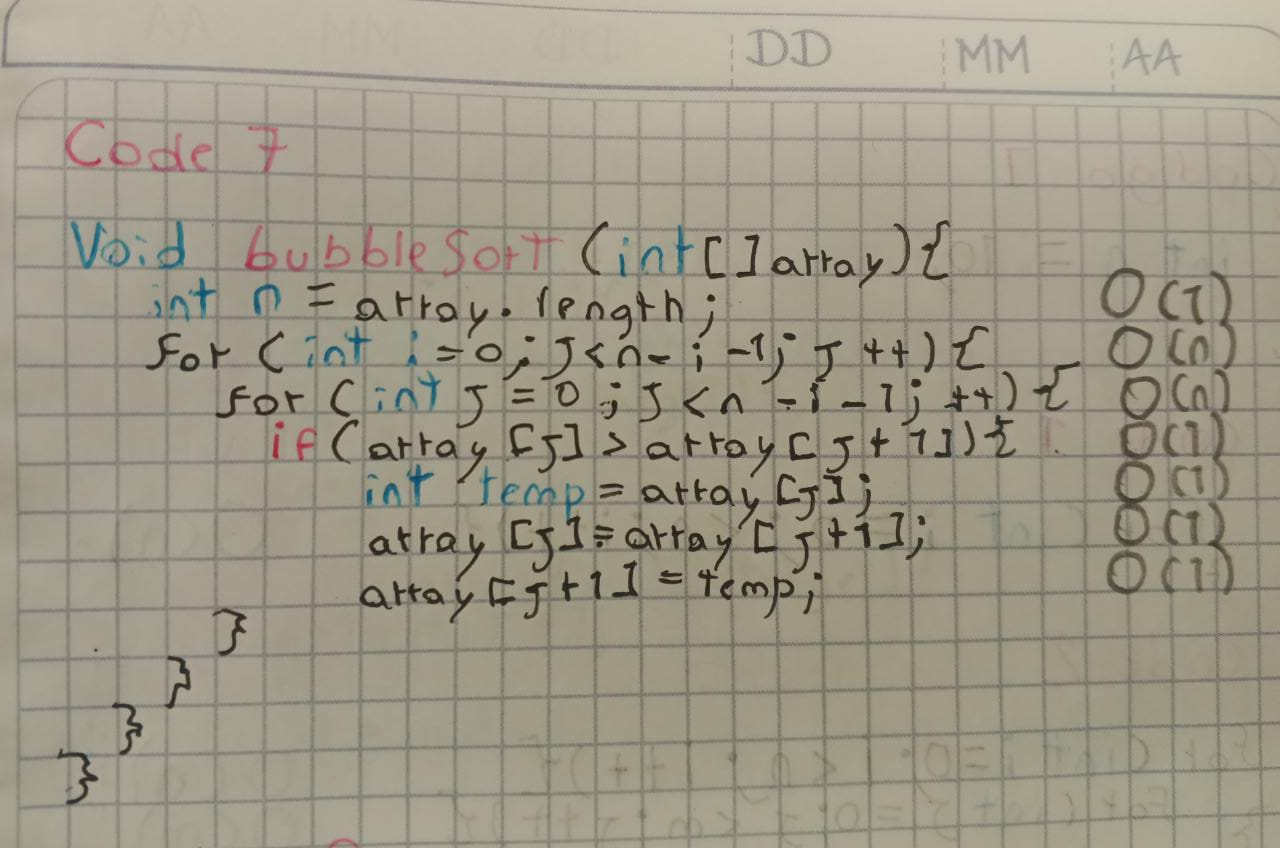
\includegraphics[width=0.4\textwidth]{WhatsApp Image 2023-09-11 at 8.00.43 PM.jpeg}
  \caption{Ejemplo código 7}
  \label{fig:imagen1}
\end{figure}

\subsection{Código número ocho}
1. La línea  calcula la longitud del arreglo `array`, lo cual es una operación de tiempo constante: O(1).

2. El bucle externo veces en el peor caso, ya que en cada iteración se coloca el elemento más pequeño en la posición correcta. La complejidad de este bucle es O(n).

3. Dentro del bucle externo, se inicializa `minIndex` en cada iteración, lo cual es una operación de tiempo constante: O(1).

4. El bucle interno desde `i + 1` hasta `n-1`, lo que significa que se ejecuta n veces en la primera iteración del bucle externo, luego `n-i-2` veces en la segunda iteración, y así sucesivamente. En el peor caso lo que resulta en una complejidad de O(n^2).

5. Dentro del bucle interno, la comparación es una operación de tiempo constante: O(1).

6. Si se encuentra un nuevo mínimo en el bucle interno, se actualiza `minIndex`, lo cual es una operación de tiempo constante: O(1).

7. Fuera del bucle interno, se realiza el intercambio de elementos en el arreglo, lo cual consiste en tres operaciones de tiempo constante: O(1).\\

complejidad total de $ O(n^2)$.
\begin{figure}[H]
  \centering
  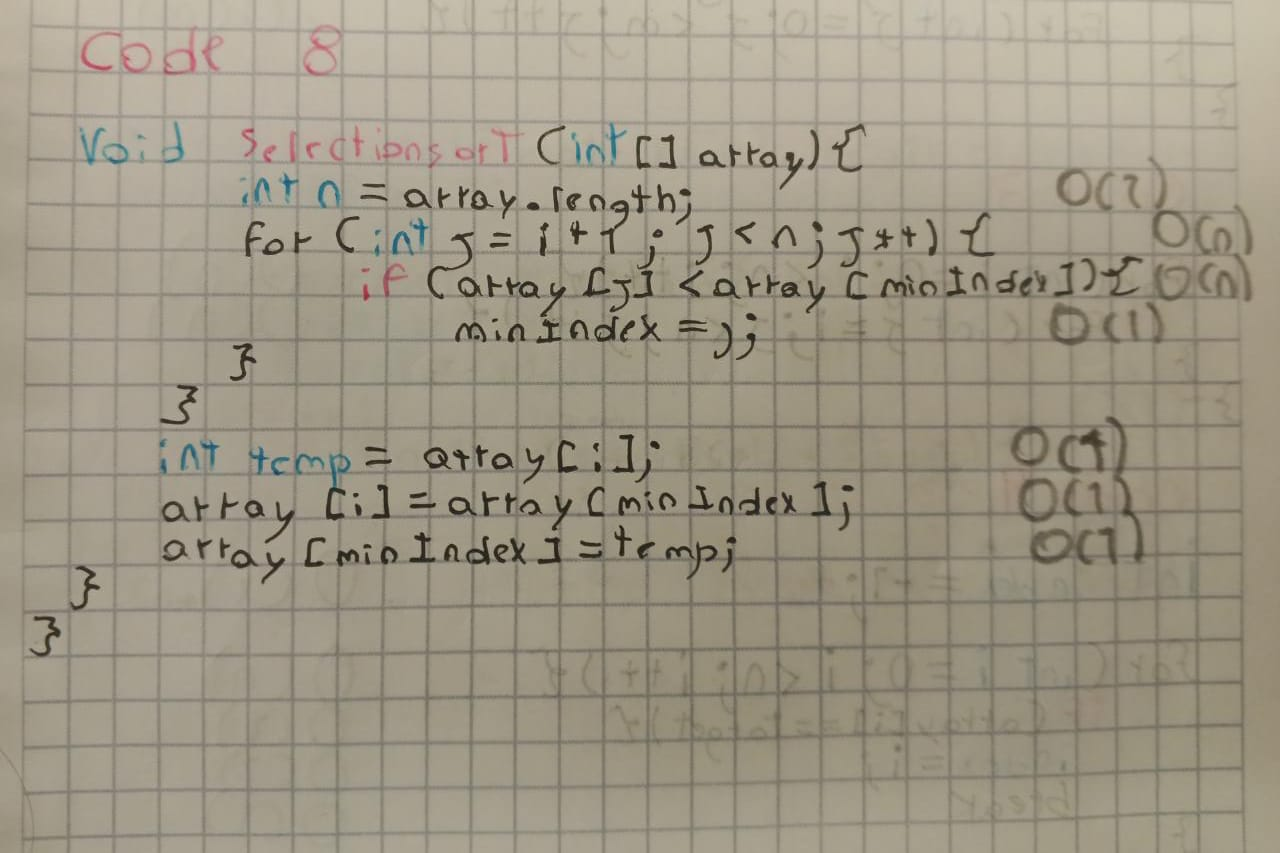
\includegraphics[width=0.4\textwidth]{WhatsApp Image 2023-09-11 at 8.01.15 PM.jpeg}
  \caption{Ejemplo código 8}
  \label{fig:imagen1}
\end{figure}

\subsection{Código número nueve}
1. La línea calcula la longitud del arreglo `array`, lo cual es una operación de tiempo constante: O(1).

2. El bucle externo for La complejidad de este bucle es O(n).

3. Dentro del bucle externo, se asigna el valor de array lo cual es una operación de tiempo constante: O(1).

4. Se inicializa  lo cual es una operación de tiempo constante: O(1).

5. El bucle interno `while  puede ejecutarse hasta `n` veces en total en todas La complejidad del bucle interno es O(n) .

6. Dentro del bucle interno, se realiza la asignación array que es una operación de tiempo constante: O(1).

7. También dentro del bucle interno, se decrementa `j` en `j--;`, lo cual es una operación de tiempo constante: O(1).

8. Finalmente, se asigna `key` a `array[j + 1]`, lo cual es una operación de tiempo constante: O(1).\\


Complejidad de O(n)\\


\begin{figure}[H]
  \centering
  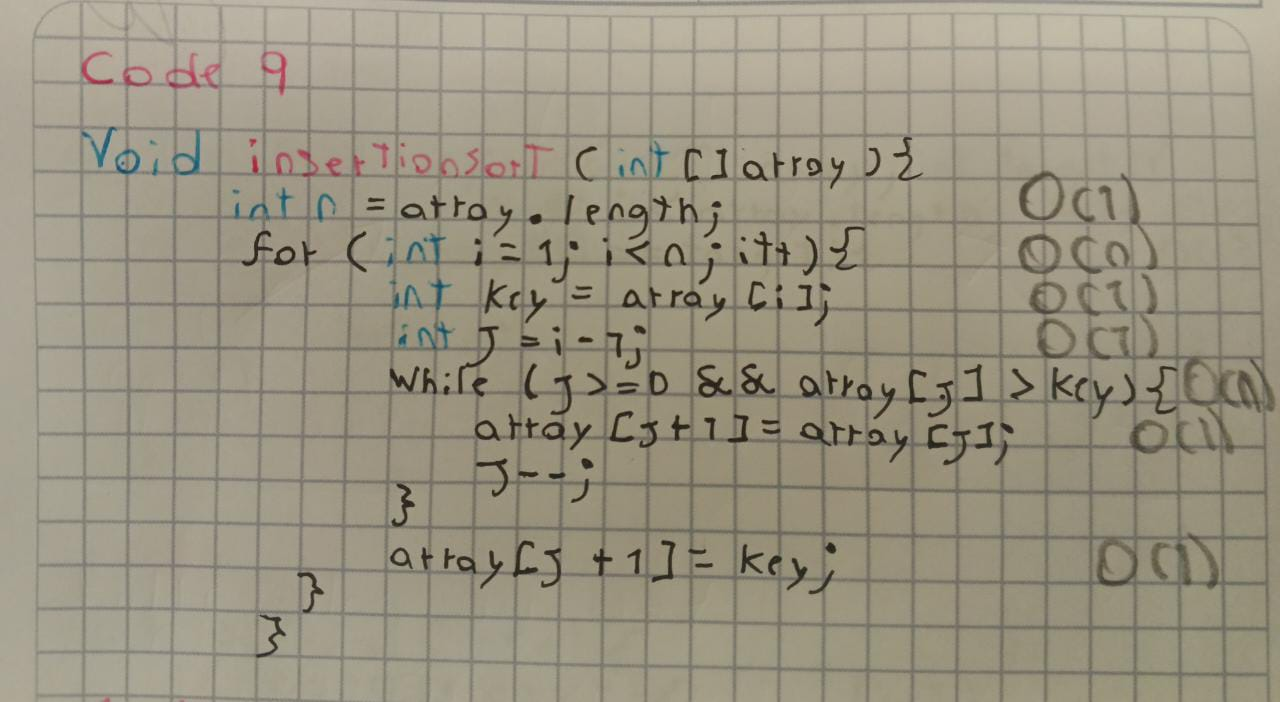
\includegraphics[width=0.4\textwidth]{WhatsApp Image 2023-09-11 at 8.01.42 PM.jpeg}
  \caption{Ejemplo código 9}
  \label{fig:imagen1}
  
  
\end{figure}\\

\subsection{Código número diez}
1. La línea `if (left < right)` es una comparación de tiempo constante: O(1).

2. La línea `int mid = left + (right - left) / 2;` calcula el índice medio `mid` del subarreglo actual y es una operación de tiempo constante: O(1).

3. Luego, la función `mergeSort` se llama recursivamente dos veces: una vez para el subarreglo izquierdo (desde `left` hasta `mid`) y una vez para el subarreglo derecho (desde `mid + 1` hasta `right`). Cada llamada recursiva divide el arreglo en dos mitades, lo que resulta en un árbol de recursión binario. En el peor caso, este árbol tiene una profundidad de `log2(n)`, donde `n` es el tamaño del arreglo original.

4. Finalmente, se llama a la función `merge` para combinar (mezclar) los subarreglos ordenados. La complejidad de la función de mezcla depende de la longitud de los subarreglos a mezclar, pero en el peor caso, se ejecutan un total de `n` operaciones, donde `n` es el tamaño del arreglo original. O(n log n) \\

Complejidad de O(n log n)
\begin{figure}[H]
  \centering
  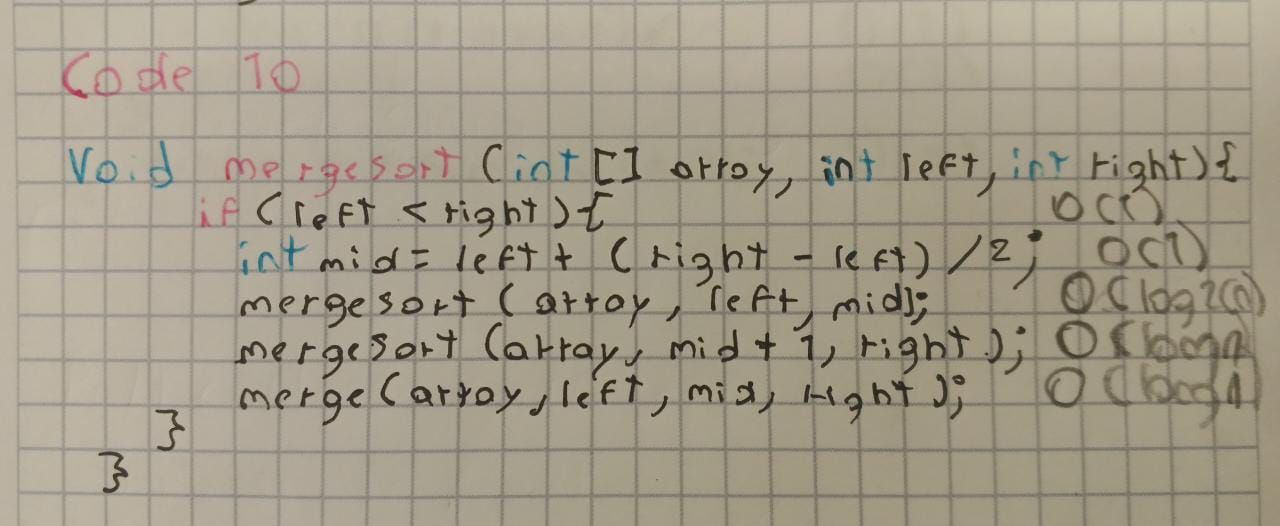
\includegraphics[width=0.4\textwidth]{WhatsApp Image 2023-09-11 at 8.02.28 PM.jpeg}
  \caption{Ejemplo código 10}
  \label{fig:imagen1}
\end{figure}

\subsection{Código número once}
1. La línea `if (low < high)` es una comparación de tiempo constante: O(1).

2. Luego, se llama a la función `partition` para realizar la partición del subarreglo. La complejidad de esta partición depende de la elección del pivote y de cómo se realiza la partición, pero en el peor caso, si el pivote no divide el arreglo en partes iguales, la partición puede ser O(n) en tiempo. Sin embargo, en promedio, se espera que la partición divida el arreglo en aproximadamente dos mitades, lo que resultaría en un tiempo de ejecución promedio de O(n log n).

3. Después de la partición, se realiza la llamada recursiva a `quickSort` en la parte izquierda (elementos menores que el pivote) y en la parte derecha (elementos mayores que el pivote). Cada una de estas llamadas recursivas se realiza en un subarreglo más pequeño y, en el peor caso, cuando no hay una partición equitativa, pueden ser hasta O(n) cada una.\\

Complejidad de O(n)


\begin{figure}[H]
  \centering
  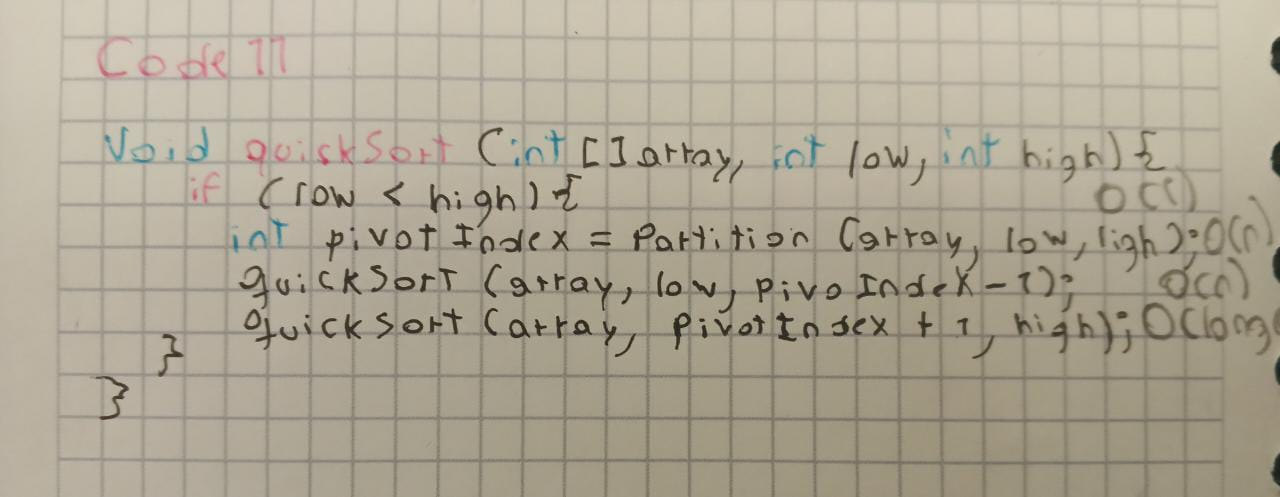
\includegraphics[width=0.4\textwidth]{WhatsApp Image 2023-09-11 at 8.02.41 PM.jpeg}
  \caption{Ejemplo código 11}
  \label{fig:imagen1}
\end{figure}

\subsection{Código número doce}
1. La línea `if (n <= 1)` es una comparación de tiempo constante y el retorno en ese caso también es de tiempo constante: O(1).

2. La creación del arreglo `dp` de longitud `n + 1` es una operación de tiempo lineal en relación con `n`: O(n).

3. Las asignaciones `dp[0] = 0;` y `dp[1] = 1;` son de tiempo constante: O(1).

4. El bucle `for (int i = 2; i <= n; i++)` itera `n-1` veces en el peor caso, ya que comienza en `i = 2` y va hasta `n`. La complejidad de este bucle es O(n).

5. Dentro del bucle, la asignación `dp[i] = dp[i - 1] + dp[i - 2];` es de tiempo constante: O(1).

6. Finalmente, el retorno `dp[n]` es una operación de tiempo constante: O(1).\\

Complejidad de O(n)


\begin{figure}[H]
  \centering
  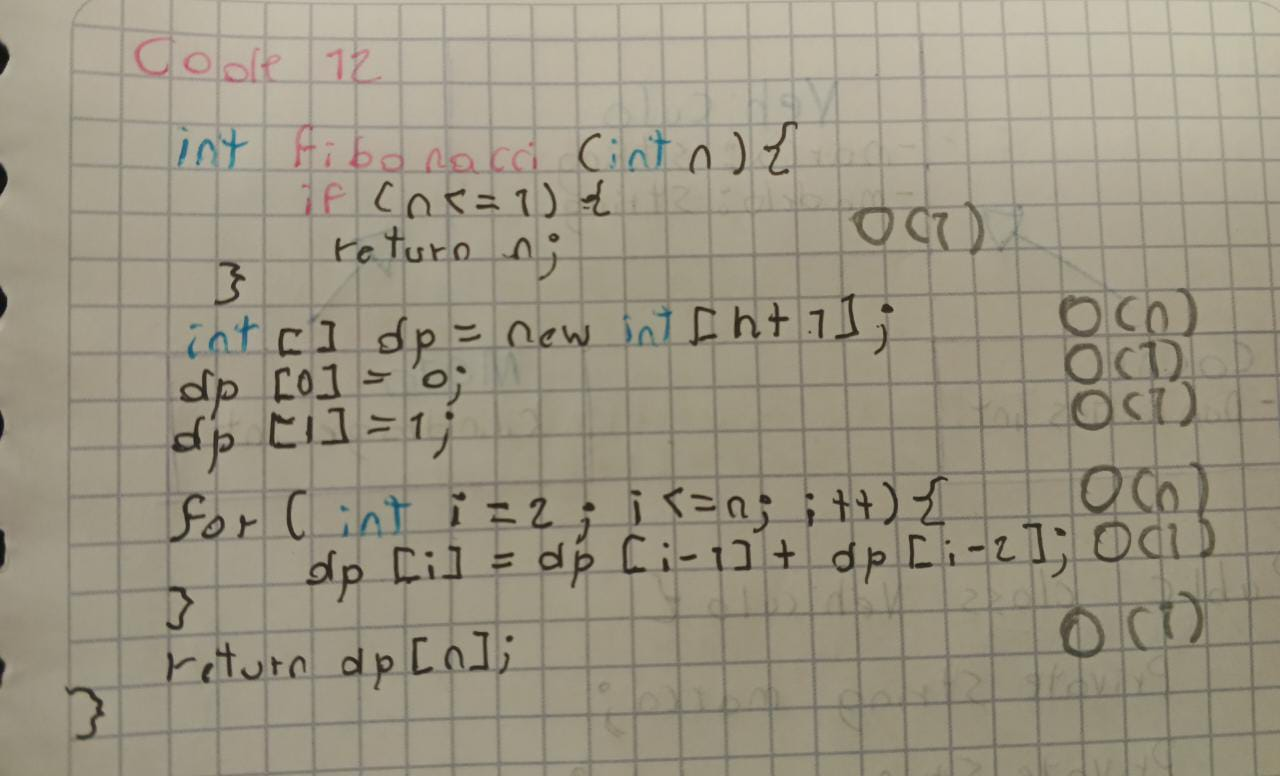
\includegraphics[width=0.4\textwidth]{WhatsApp Image 2023-09-11 at 8.02.55 PM.jpeg}
  \caption{Ejemplo código 12}
  \label{fig:imagen1}
\end{figure}

\subsection{Código número trece}
1. El bucle `for (int i = 0; i < array.length; i++)` itera a través de cada elemento en el arreglo `array`. En el peor caso, si el valor `target` no se encuentra en el arreglo y es necesario recorrer todo el arreglo hasta el final, este bucle se ejecutará `n` veces, donde `n` es la longitud del arreglo. La complejidad de este bucle es O(n) en el peor caso.

2. Dentro del bucle, la comparación `if (array[i] == target)` es una operación de tiempo constante, ya que simplemente compara dos valores: O(1).\\

Complejidad de O(n)


\begin{figure}[H]
  \centering
  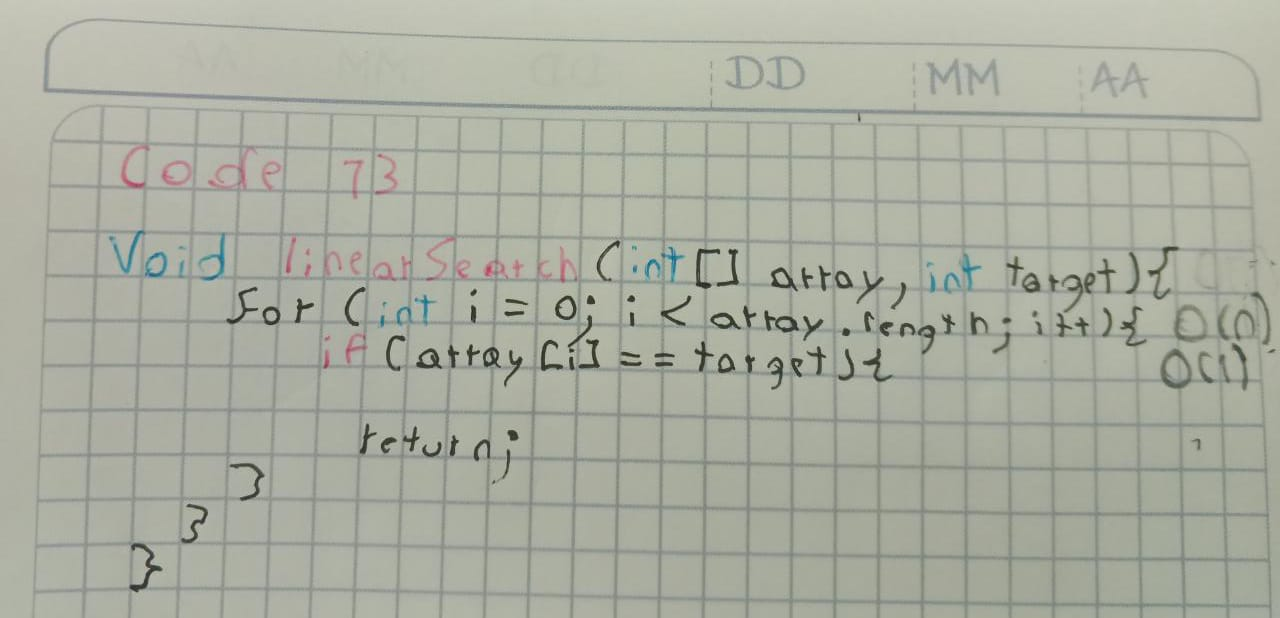
\includegraphics[width=0.4\textwidth]{WhatsApp Image 2023-09-11 at 8.03.21 PM (1).jpeg}
  \caption{Ejemplo código 13}
  \label{fig:imagen1}
\end{figure}

\subsection{Código número catorce}
1. Las asignaciones `int left = 0` y `int right = sortedArray.length - 1` son operaciones de tiempo constante: O(1).

2. El bucle `while (left <= right)` implementa la búsqueda binaria. En el peor caso, este bucle se ejecutará hasta que `left` sea mayor que `right`. La búsqueda binaria tiene una complejidad de tiempo de O(log n) en el peor caso, donde `n` es la longitud del arreglo.

3. La línea `int mid = left + (right - left) / 2;` calcula el índice medio `mid` del rango actual. Esta operación es de tiempo constante: O(1).

4. La comparación `if (sortedArray[mid] == target)` es una operación de tiempo constante y se ejecuta en el peor caso una vez: O(1).

5. Las asignaciones `left = mid + 1;` y `right = mid - 1;` son operaciones de tiempo constante que también se ejecutan en el peor caso una vez: O(1).

6. El retorno `mid` cuando se encuentra el elemento es de tiempo constante: O(1).

7. Si el elemento no se encuentra y el bucle se ejecuta hasta que `left` sea mayor que `right`, el retorno `-1` indicando que el elemento no se encontró también es de tiempo constante: O(1).\\

Complejidad de O(n log n)

\begin{figure}[H]
  \centering
  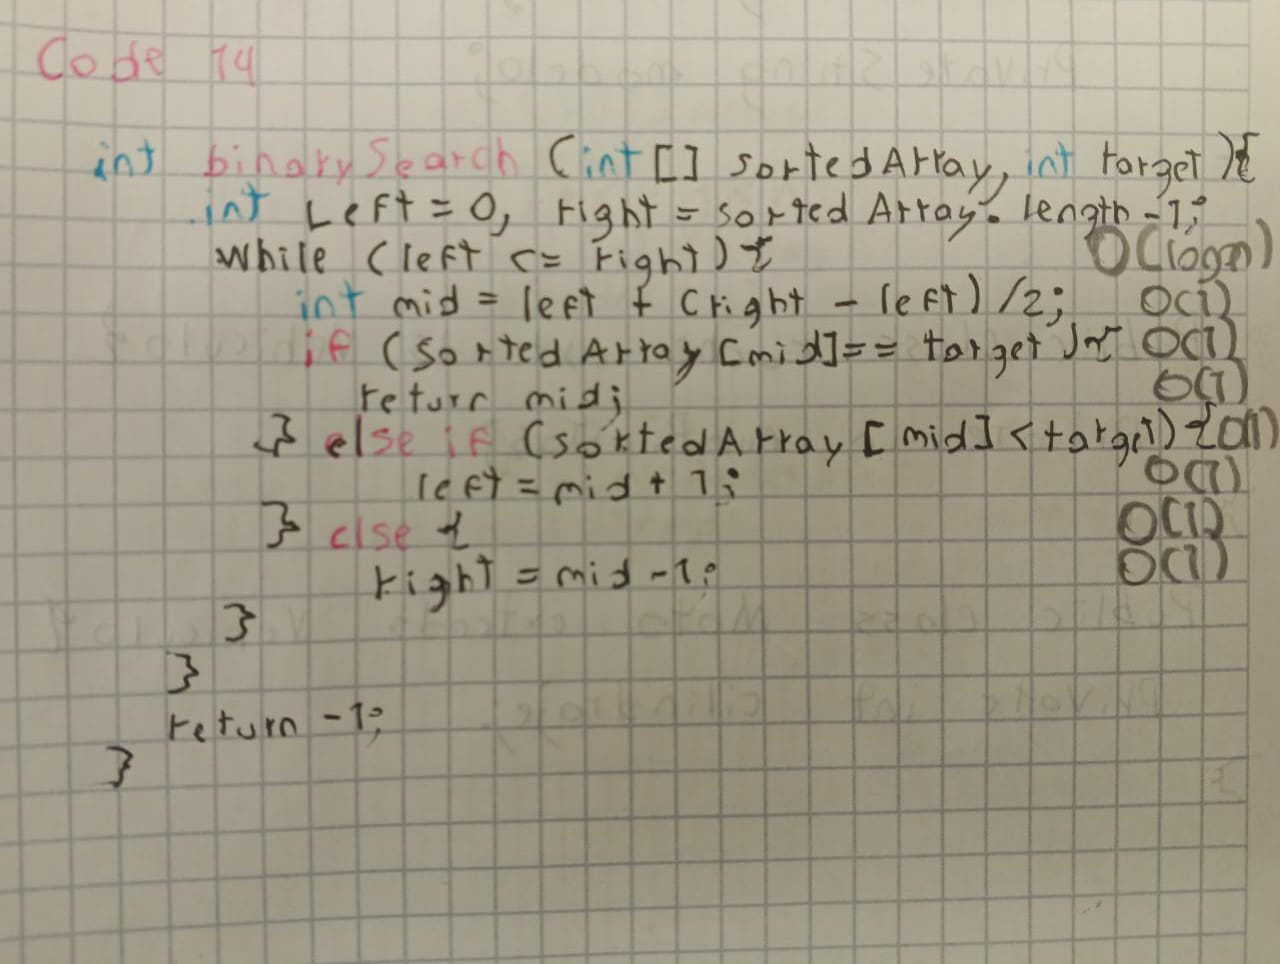
\includegraphics[width=0.4\textwidth]{WhatsApp Image 2023-09-11 at 8.03.37 PM.jpeg}
  \caption{Ejemplo código 14}
  \label{fig:imagen1}
\end{figure}

\subsection{Código número quince}
1. La condición `if (n == 0 || n == 1)` es una operación de tiempo constante, ya que simplemente verifica si `n` es igual a 0 o 1: O(1).

2. El retorno `1` cuando `n` es 0 o 1 también es una operación de tiempo constante: O(1).

3. La llamada recursiva `return n * factorial(n - 1);` es el corazón de la función y es donde ocurre la recursión. Cada vez que se realiza una llamada recursiva, `n` se decrementa en 1 hasta llegar a 1 o 0, momento en el cual se detiene la recursión. En el peor caso, esto implica que la función se llama `n` veces antes de alcanzar el caso base. Por lo tanto, la complejidad de tiempo de esta llamada recursiva es O(n) en el peor caso.\\

Complejidad de O(n)

\begin{figure}[H]
  \centering
  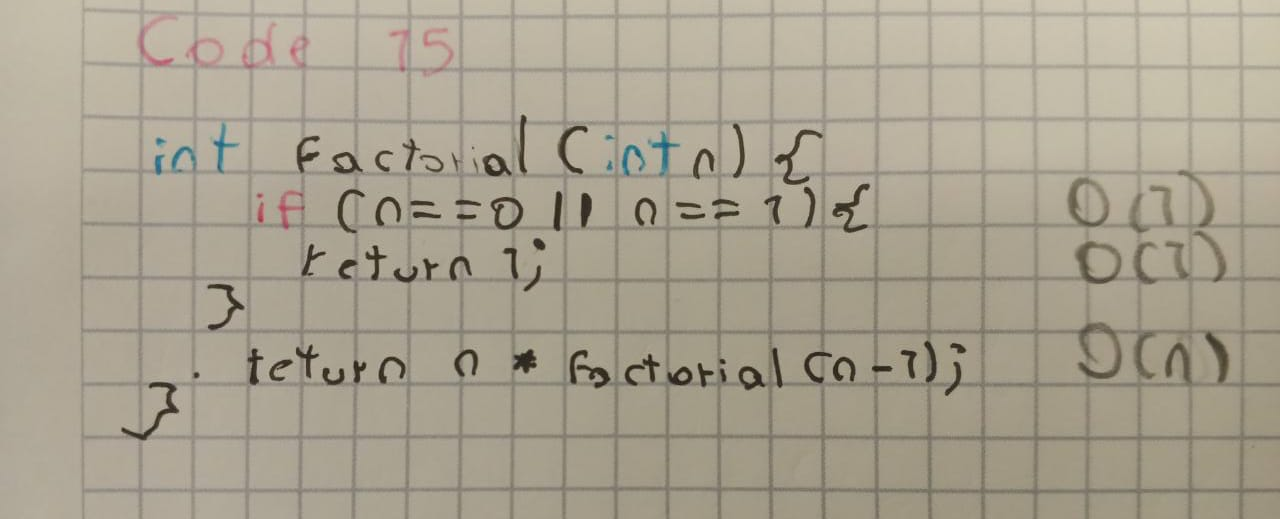
\includegraphics[width=0.4\textwidth]{WhatsApp Image 2023-09-11 at 8.03.47 PM.jpeg}
  \caption{Ejemplo código 15}
  

  \label{fig:imagen1}
\end{figure}

\section{Conclusiones}


En este estudio, evaluamos la complejidad de varios algoritmos mediante la notación Big-O. Descubrimos que su eficiencia varía ampliamente: algunos son lineales (O(n)), otros cuadráticos (O(n^2)), y algunos logarítmicos (O(log n)).

Este análisis resalta la importancia de seleccionar algoritmos adecuados para diferentes tareas, considerando el tamaño de los conjuntos de datos. La notación Big-O proporciona una herramienta esencial para tomar decisiones fundamentadas sobre la eficiencia de los algoritmos.

\end{document}